\section{Inter-server Communication}
As described earlier, inter-server communication, the ability to play the game with other users on other servers with different implementations, will be achieved using ReST. The full API set for the ReST protocol is dependent on other groups and as of writing is currently under discussion.
\\As the API is incomplete, it is not possible to fully describe all the functionality of the service. But this section gives an example of how ReST will work for friendships between users on foreign servers.
\\
\\
As per the the Requirements Specification, there should be a way to send, accept and reject friend requests between servers, and to be able to manage a users list of friends (i.e. deleting confirmed friendships).\\
For friendships to work across servers, the programs need to know the IDs of both users and the ID of the other server (so one server knows where to find the “remote” user).\\
Whilst there is no requirement for secure authentication between users, there can be a simple ‘handshaking’ protocol simply to prevent (read: make it harder for) anyone from explicitly saying that they are friends with a user when that user has not agreed to be friends with them.\\
%Data is “mirrored” on either server. For example, the “local user” on one server, will be the “remote user” on the other server.\\
%\\
%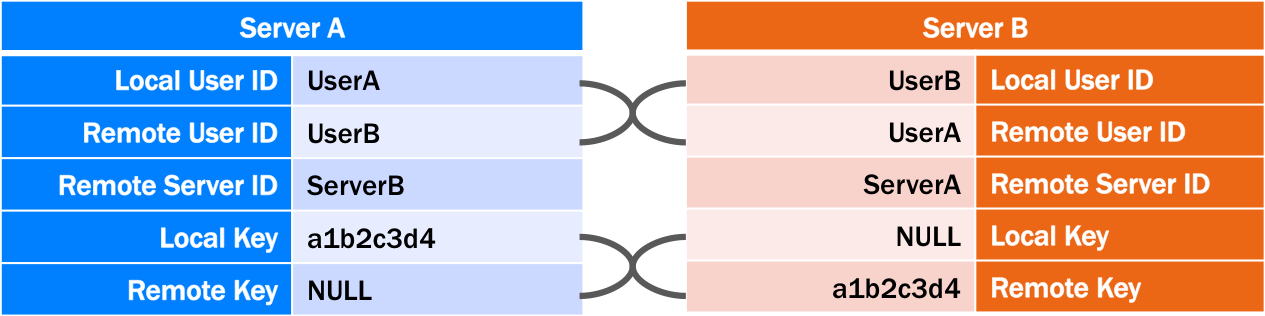
\includegraphics[scale=0.75]{img/FriendshipEntity.png}

\paragraph{Key exchange handshake authentication}
The basic premise of friendship authentication is to exchange “keys”.
Each friendship has two keys, one key per user on their server.
To interact with a user (i.e. fight their monsters), you need to know their key which they generated, and vice versa, for them to interact with you, they need your key for that friendship.
\paragraph{Friend request life cycle}
The status of whether a friendship is accepted is defined simply as whether both servers have keys for each other.
When a friend request is sent, a key for the server that is sending the request is supplied, but there is no key from the other server. To accept the friend request, the server generates a key, stores it, then sends that key back to the other server.
Now both servers have keys for the friendship, and both servers know both keys, so they can talk to each other.
\\
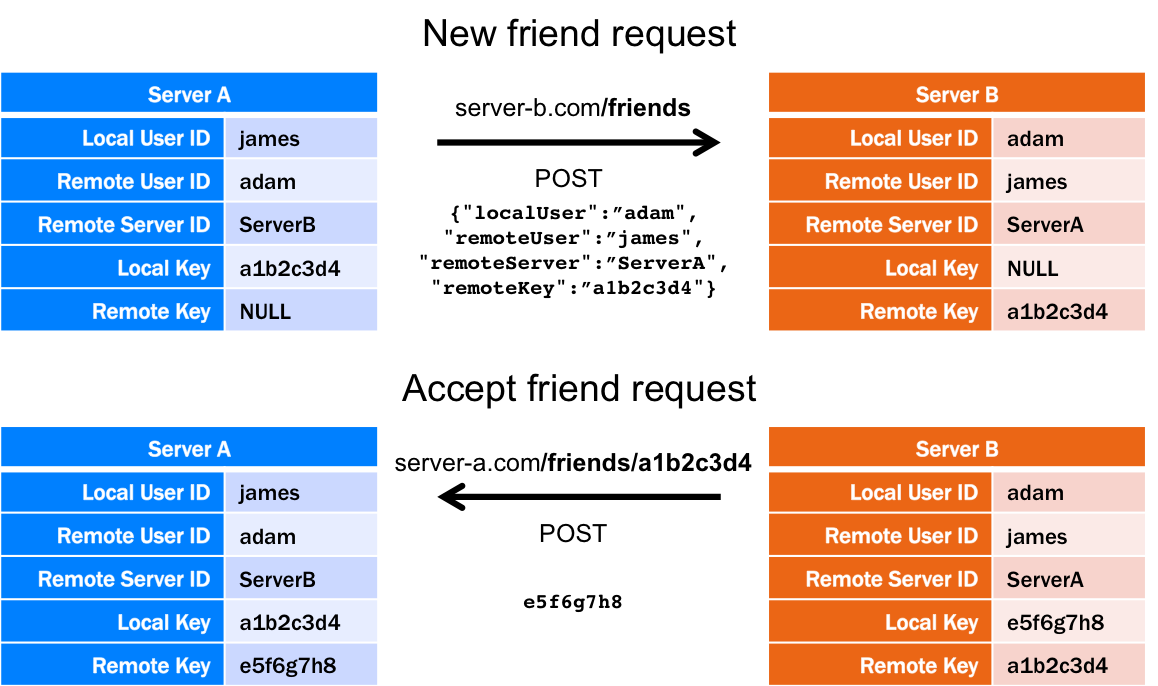
\includegraphics[scale=0.85]{img/FriendshipRESTCycle.png} 
